\qrchapter{https://forgottenpillar.com/rsc/en-fp-chapter4}{Revision of “Living Temple”}


\qrchapter{https://forgottenpillar.com/rsc/en-fp-chapter4}{Revisión de “Living Temple”}


In \textit{Testimonies for the Church Containing Letters to Physicians and Ministers Instruction to Seventh-Day Adventists}, the tenth chapter, \textit{The Foundation of our Faith,} God gave valuable lessons on the development and consequences of Kellogg's theories. The broader and deeper meaning of these quotations can be understood when we are familiar with their historical context. Let us first take a brief look at the historical context of Kellogg's book, The \textit{Living Temple}.


En \textit{Testimonios para la Iglesia que contienen cartas a los médicos y a los ministros de instrucción a los adventistas del séptimo día}, el décimo capítulo, \textit{El fundamento de nuestra fe}, Dios dio valiosas lecciones sobre el desarrollo y las consecuencias de las teorías de Kellogg. El significado más amplio y profundo de estas citas puede entenderse cuando nos familiarizamos con su contexto histórico. Veamos primero brevemente el contexto histórico del libro de Kellogg, \textit{The Living Temple}.


In a series of providence, God signified that “\textit{Living Temple}” should not be printed. One such event was the burning of Battle Creek's press building, just the night before it was to be printed. Finally, the book was printed elsewhere; it instigated a great crisis in the Seventh-day Adventist Church. On October 7, 1903, a annual meeting of the conference was held in Washington DC. Many Seventh-day Adventist church leaders were present, including Dr. Kellogg and his sympathizers. Major controversy was taking place over this book and the conflict was inevitable. Fortunately, on the brink of this escalating conflict, a letter from Sister White was delivered to the council. On Sunday, the letter fell upon the ears of all, to which there resounded many “amen's” and “halleluyah's”. It was a very tense and moving morning for the church that was on the verge of a split—to at last have concrete direction from the Lord's messenger:


En una serie de providencias, Dios indicó que “\textit{Living Temple}” no debía imprimirse. Una de ellas fue el incendio del edificio de la imprenta de Battle Creek, justo la noche antes de que se imprimiera. Finalmente, el libro se imprimió en otro lugar; provocó una gran crisis en la Iglesia Adventista del Séptimo Día. El 7 de octubre de 1903, se celebró una reunión anual de la conferencia en Washington DC. Muchos líderes de la Iglesia Adventista del Séptimo Día estaban presentes, incluyendo al Dr. Kellogg y sus simpatizantes. Se estaba produciendo una gran controversia sobre este libro y el conflicto era inevitable. Afortunadamente, al borde de esta escalada del conflicto, se entregó al consejo una carta de la hermana White. El domingo, la carta cayó en los oídos de todos, a los que resonaron muchos “amén” y “aleluyas”. Fue una mañana muy tensa y conmovedora para la iglesia, que estaba al borde de la ruptura—al tener por fin una dirección concreta del mensajero del Señor:


\begin{figure}[h]
    \centering
    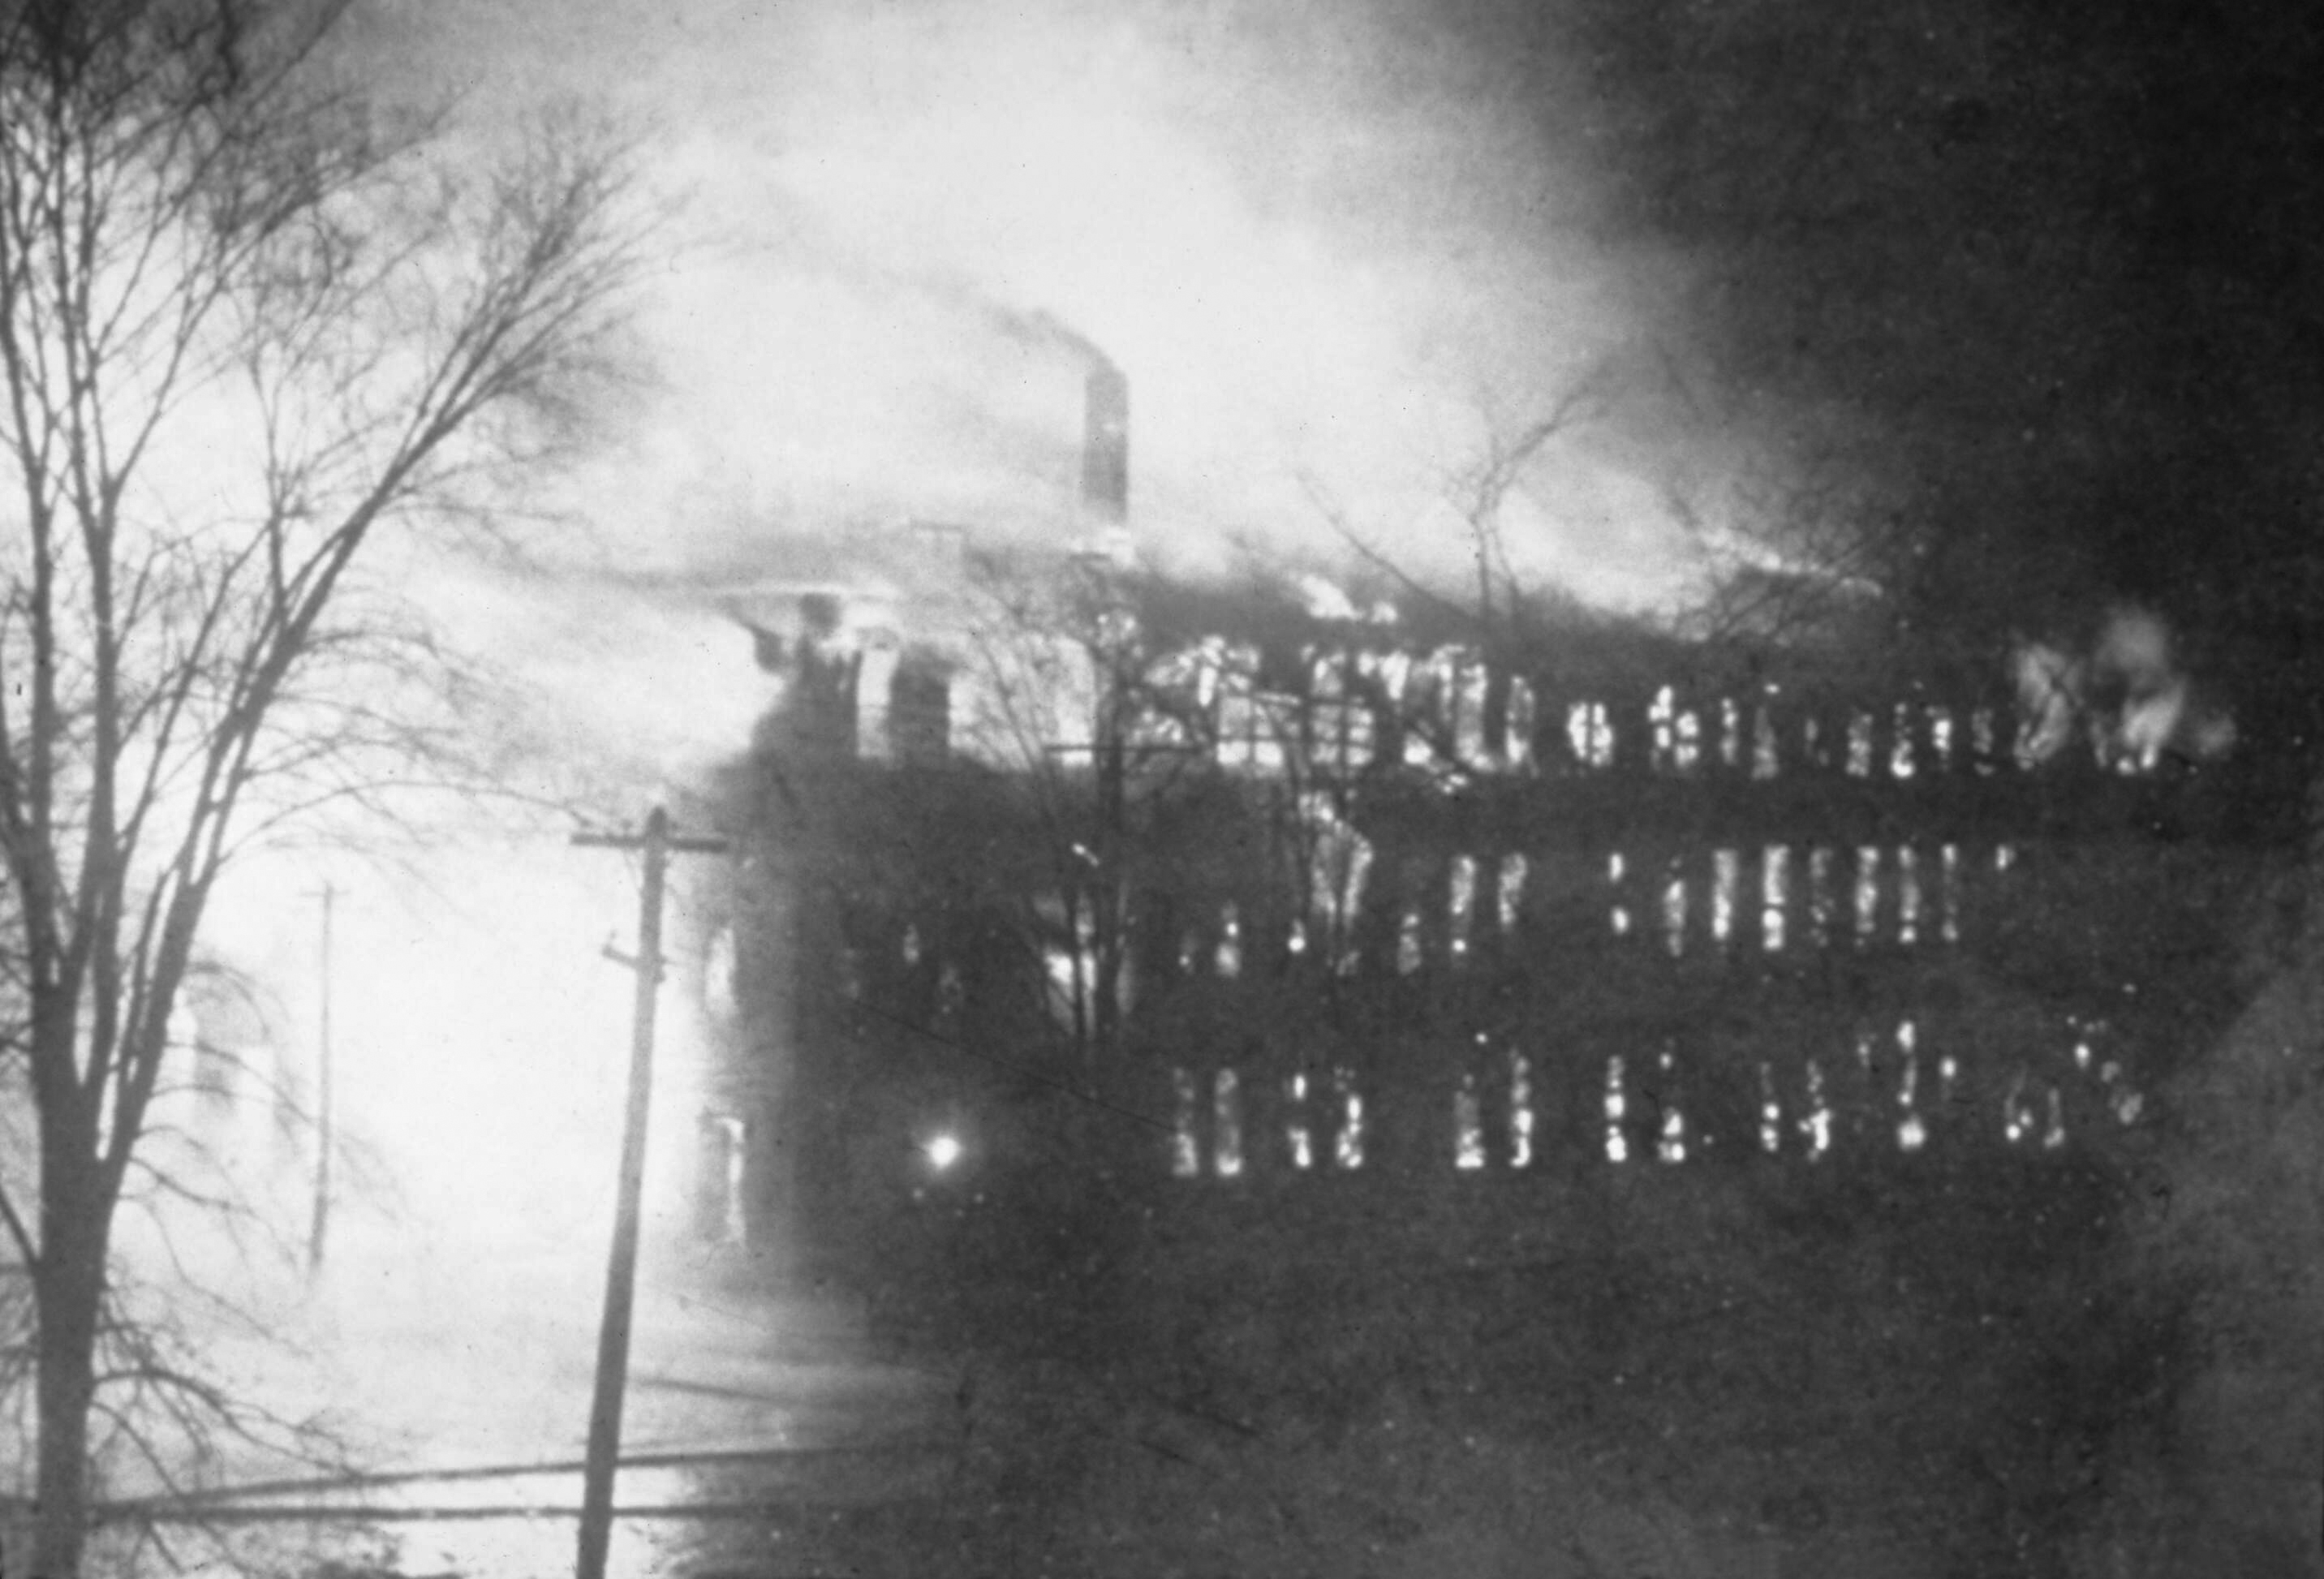
\includegraphics[width=1\linewidth]{images/review-and-herlad.jpg}
    \caption*{Burning of Review and Herald press building, December 30, 1902.}
    \label{fig:review-and-herald}
\end{figure}


\begin{figure}[h]
    \centering
    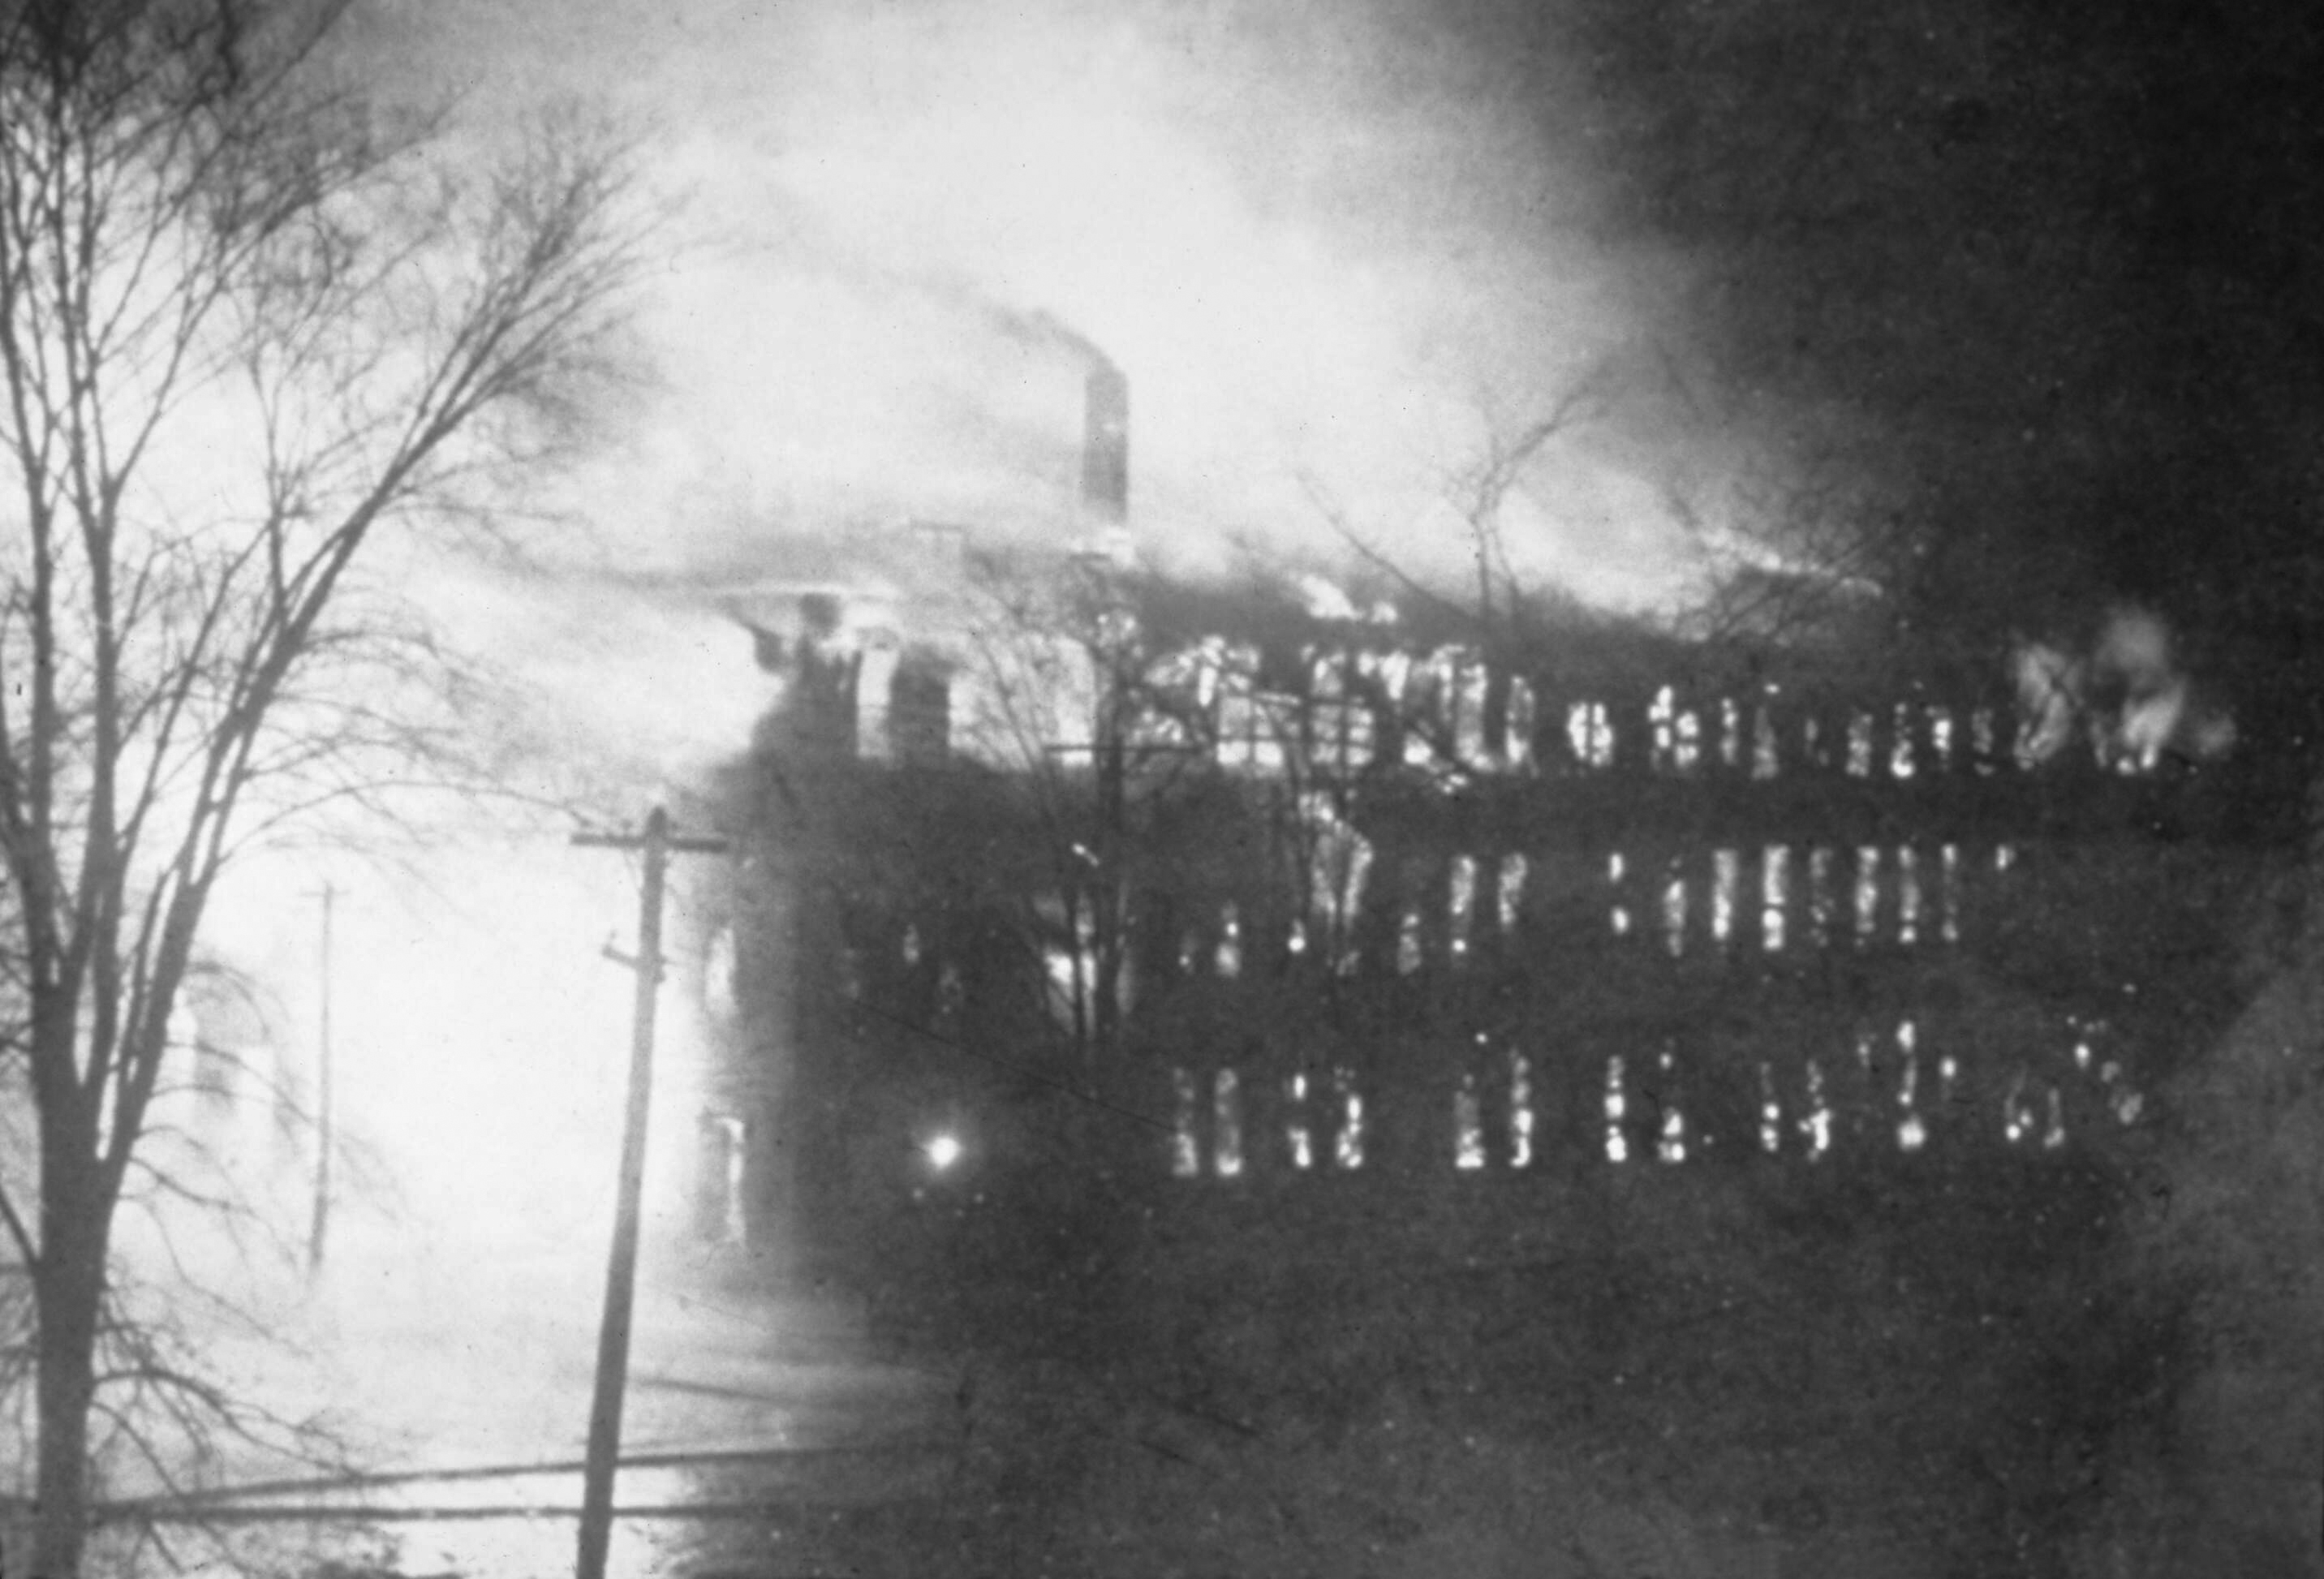
\includegraphics[width=1\linewidth]{images/review-and-herlad.jpg}
    \caption*{Incendio del edificio de la imprenta Review and Herald, 30 de diciembre de 1902.}
    \label{fig:review-and-herald}
\end{figure}


\egw{I have some things to say to our teachers in reference to \textbf{the new book The Living Temple}. \textbf{Be careful how you sustain \underline{the sentiments of this book regarding the personality of God}}. As the Lord presents matters to me, \textbf{these sentiments do not bear the endorsement of God}. \textbf{They are a snare that the enemy has prepared for these last days}. I thought that this would surely be discerned and that it would not be necessary for me to say anything about it. \textbf{But since the claim has been made that the teachings of this book can be sustained by statements from my writings, I am compelled to speak in denial of this claim}. There may be in this book expressions and sentiments that are in harmony with my writings. And there may be in my writings many statements which when taken from their connection, and interpreted according to the mind of the writer of Living Temple, would seem to be in harmony with the teachings of this book. \textbf{This may give apparent support to the assertion that the sentiments in Living Temple are in harmony with my writings}. \textbf{But God forbid that this opinion should prevail}.}[Lt211-1903.1; 1903][https://egwwritings.org/read?panels=p14068.9598008]


\egw{Tengo algunas cosas que decir a nuestros maestros en referencia al \textbf{nuevo libro The Living Temple}. \textbf{Tened cuidado de cómo sostenéis \underline{los sentimientos de este libro en relación con la personalidad de Dios}}. Tal como el Señor me presenta los asuntos, \textbf{estos sentimientos no llevan el respaldo de Dios}. \textbf{Son una trampa que el enemigo ha preparado para estos últimos días}. Pensé que esto sería seguramente discernido y que no sería necesario que yo dijera nada al respecto. \textbf{Pero ya que se ha hecho la afirmación de que las enseñanzas de este libro pueden ser sostenidas por declaraciones de mis escritos, me veo obligada a hablar en negación de esta afirmación}. Puede haber en este libro expresiones y sentimientos que estén en armonía con mis escritos. Y puede haber en mis escritos muchas declaraciones que cuando se toman de su conexión, y se interpretan de acuerdo con la mente del escritor de Living Temple, parecerían estar en armonía con las enseñanzas de este libro. \textbf{Esto puede dar un apoyo aparente a la afirmación de que los sentimientos en Living Temple están en armonía con mis escritos}. \textbf{Pero Dios no permita que esta opinión prevalezca}.}[Lt211-1903.1; 1903][https://egwwritings.org/read?panels=p14068.9598008]


Repeatedly, Sister White stated that the true problem of the book was the sentiments\egwinline{\textbf{regarding the personality of God}}. These sentiments are not sustained by statements from Ellen White's writings and these very sentiments\egwinline{\textbf{are a snare that the enemy has prepared for these last days}}.


Repetidamente, la hermana White declaró que el verdadero problema del libro eran los sentimientos\egwinline{\textbf{respecto a la personalidad de Dios}}. Estos sentimientos no se sustentan en las declaraciones de los escritos de Ellen White y estos mismos sentimientos\egwinline{\textbf{son una trampa que el enemigo ha preparado para estos últimos días}}.


God, again in His providence, solved this conflict. Kellogg accepted the reproof from the Lord's messenger and, before the council closed, he stated that the Living Temple would be taken from the market\footnote{\href{https://forgottenpillar.com/wp-content/uploads/2022/04/Letter-A-G-Daniells-to-W-C-White-October-29-1903.pdf}{Letter: A. G. Daniells to W. C. White, October 23, 1903, pp. 5}}. But after the conference, he spoke privately with the general conference president, Brother Arthur G. Daniells, about his plans for revising the book. The following is a look at select letters, revealing Kellogg's plans for revising “\textit{Living Temple}”.


Dios, de nuevo en su providencia, resolvió este conflicto. Kellogg aceptó la reprimenda del mensajero del Señor y, antes de que se cerrara el concilio, declaró que El Templo Viviente sería retirado del mercado\footnote{\href{https://forgottenpillar.com/wp-content/uploads/2022/04/Letter-A-G-Daniells-to-W-C-White-October-29-1903.pdf}{Carta: A. G. Daniells a W. C. White, 23 de octubre de 1903, pp. 5}}. Pero después de la conferencia, habló en privado con el presidente de la conferencia general, el hermano Arthur G. Daniells, sobre sus planes para revisar el libro. Lo siguiente es una mirada a cartas selectas, que revelan los planes de Kellogg para revisar “\textit{Living Temple}”.


Ellen White was not present at the yearly conference in Washington DC but her son, William C. White, did attend. When the conference was over, brother Arthur G. Daniells wrote a confidential letter to William C. White regarding Dr. Kellogg's plan to revise his book:


Ellen White no estuvo presente en la conferencia anual en Washington DC, pero su hijo, William C. White, sí asistió. Cuando la conferencia terminó, el hermano Arthur G. Daniells escribió una carta confidencial a William C. White sobre el plan del Dr. Kellogg de revisar su libro:


\others{October 29, 1903}


\others{29 de octubre de 1903}


\othersnogap{Ever since the \textbf{council closed} I have felt that I should write you \textbf{confidentially regarding Dr. Kellogg's plans for revising and republishing ‘The Living Temple’}…. He \normaltext{[Kellogg]} said that some days before coming to the council, he had been thinking the matter over, and began to see that \textbf{he had made a slight mistake in expressing his views}. He said that all the way along he had been troubled to know how to state the character of God and his relation to his creation works…}


\othersnogap{Desde que \textbf{se clausuró el concilio}, he sentido que debía escribirle \textbf{confidencialmente con respecto a los planes del Dr. Kellogg para revisar y reeditar ‘El Templo Viviente’}... Él \normaltext{[Kellogg]} dijo que algunos días antes de venir al consejo, había estado pensando en el asunto, y comenzó a ver que \textbf{había cometido un ligero error al expresar sus opiniones}. Dijo que todo el tiempo había estado preocupado por saber cómo declarar el carácter de Dios y su relación con las obras de su creación...}


\begin{figure}[hp]
    \centering
    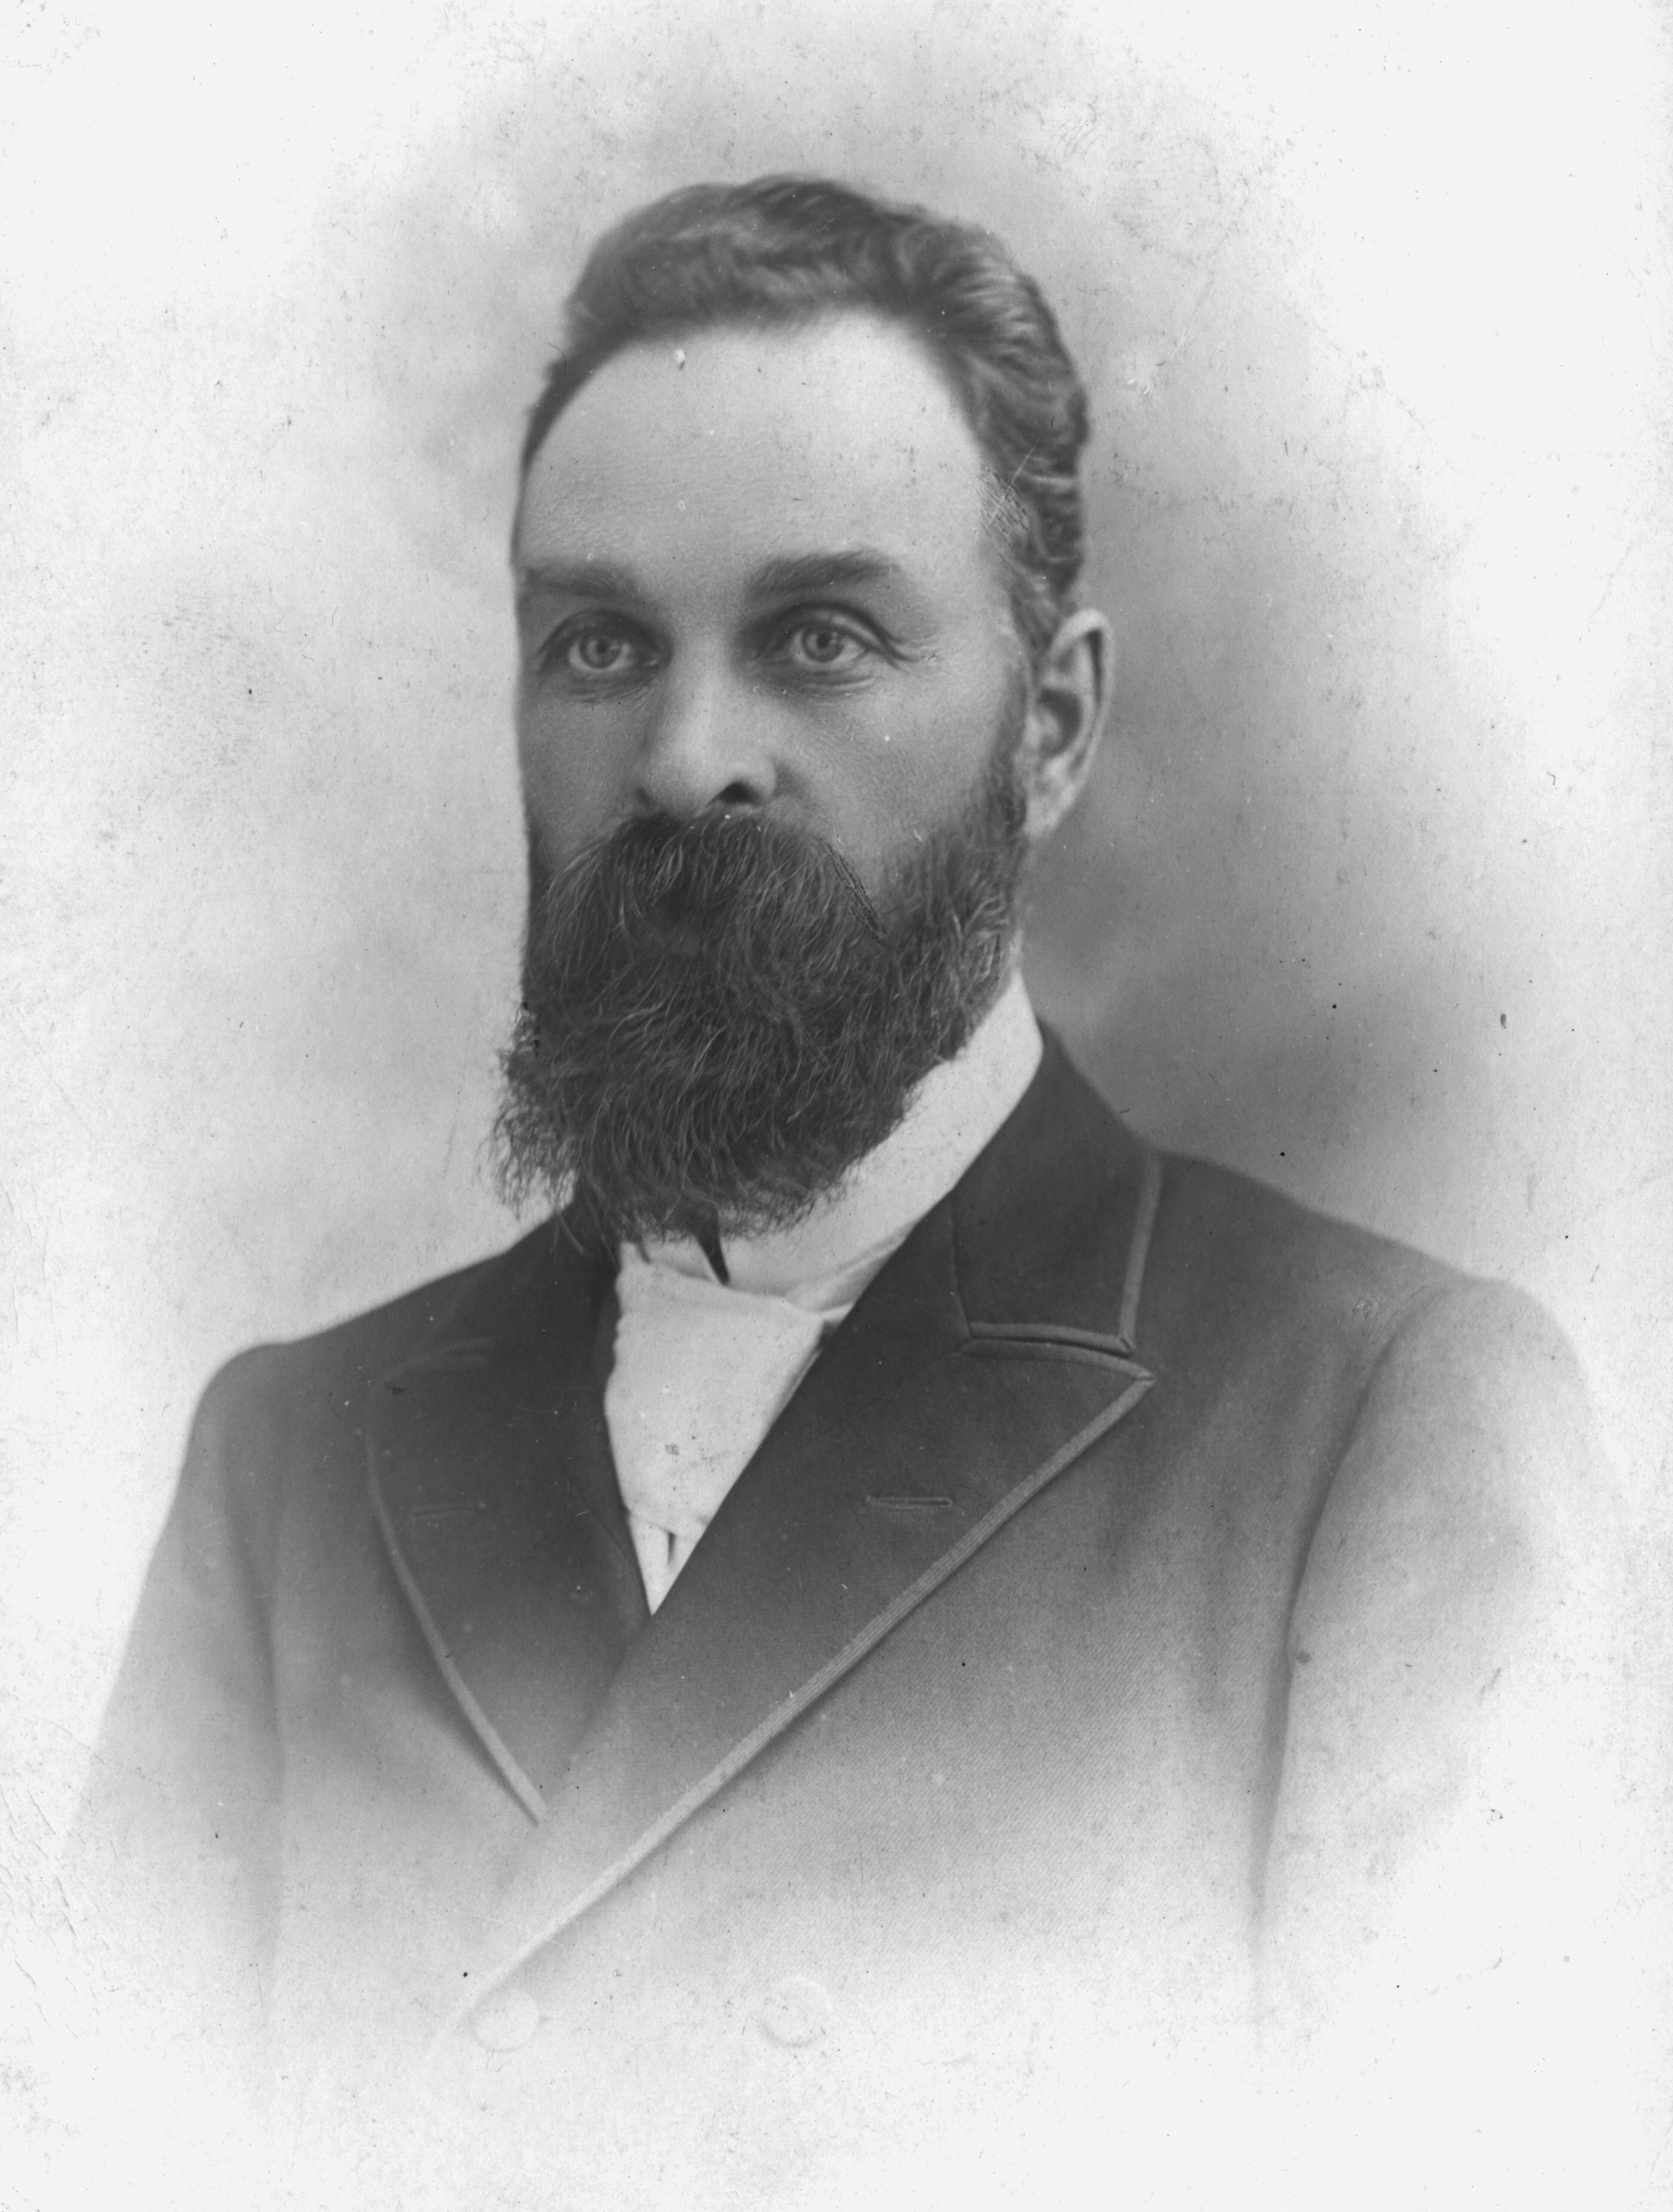
\includegraphics[width=1\linewidth]{images/daniels.jpg}
    \caption*{Arthur Grosvenor Daniells (1858-1935)}
    \label{fig:daniells}
\end{figure}


\begin{figure}[hp]
    \centering
    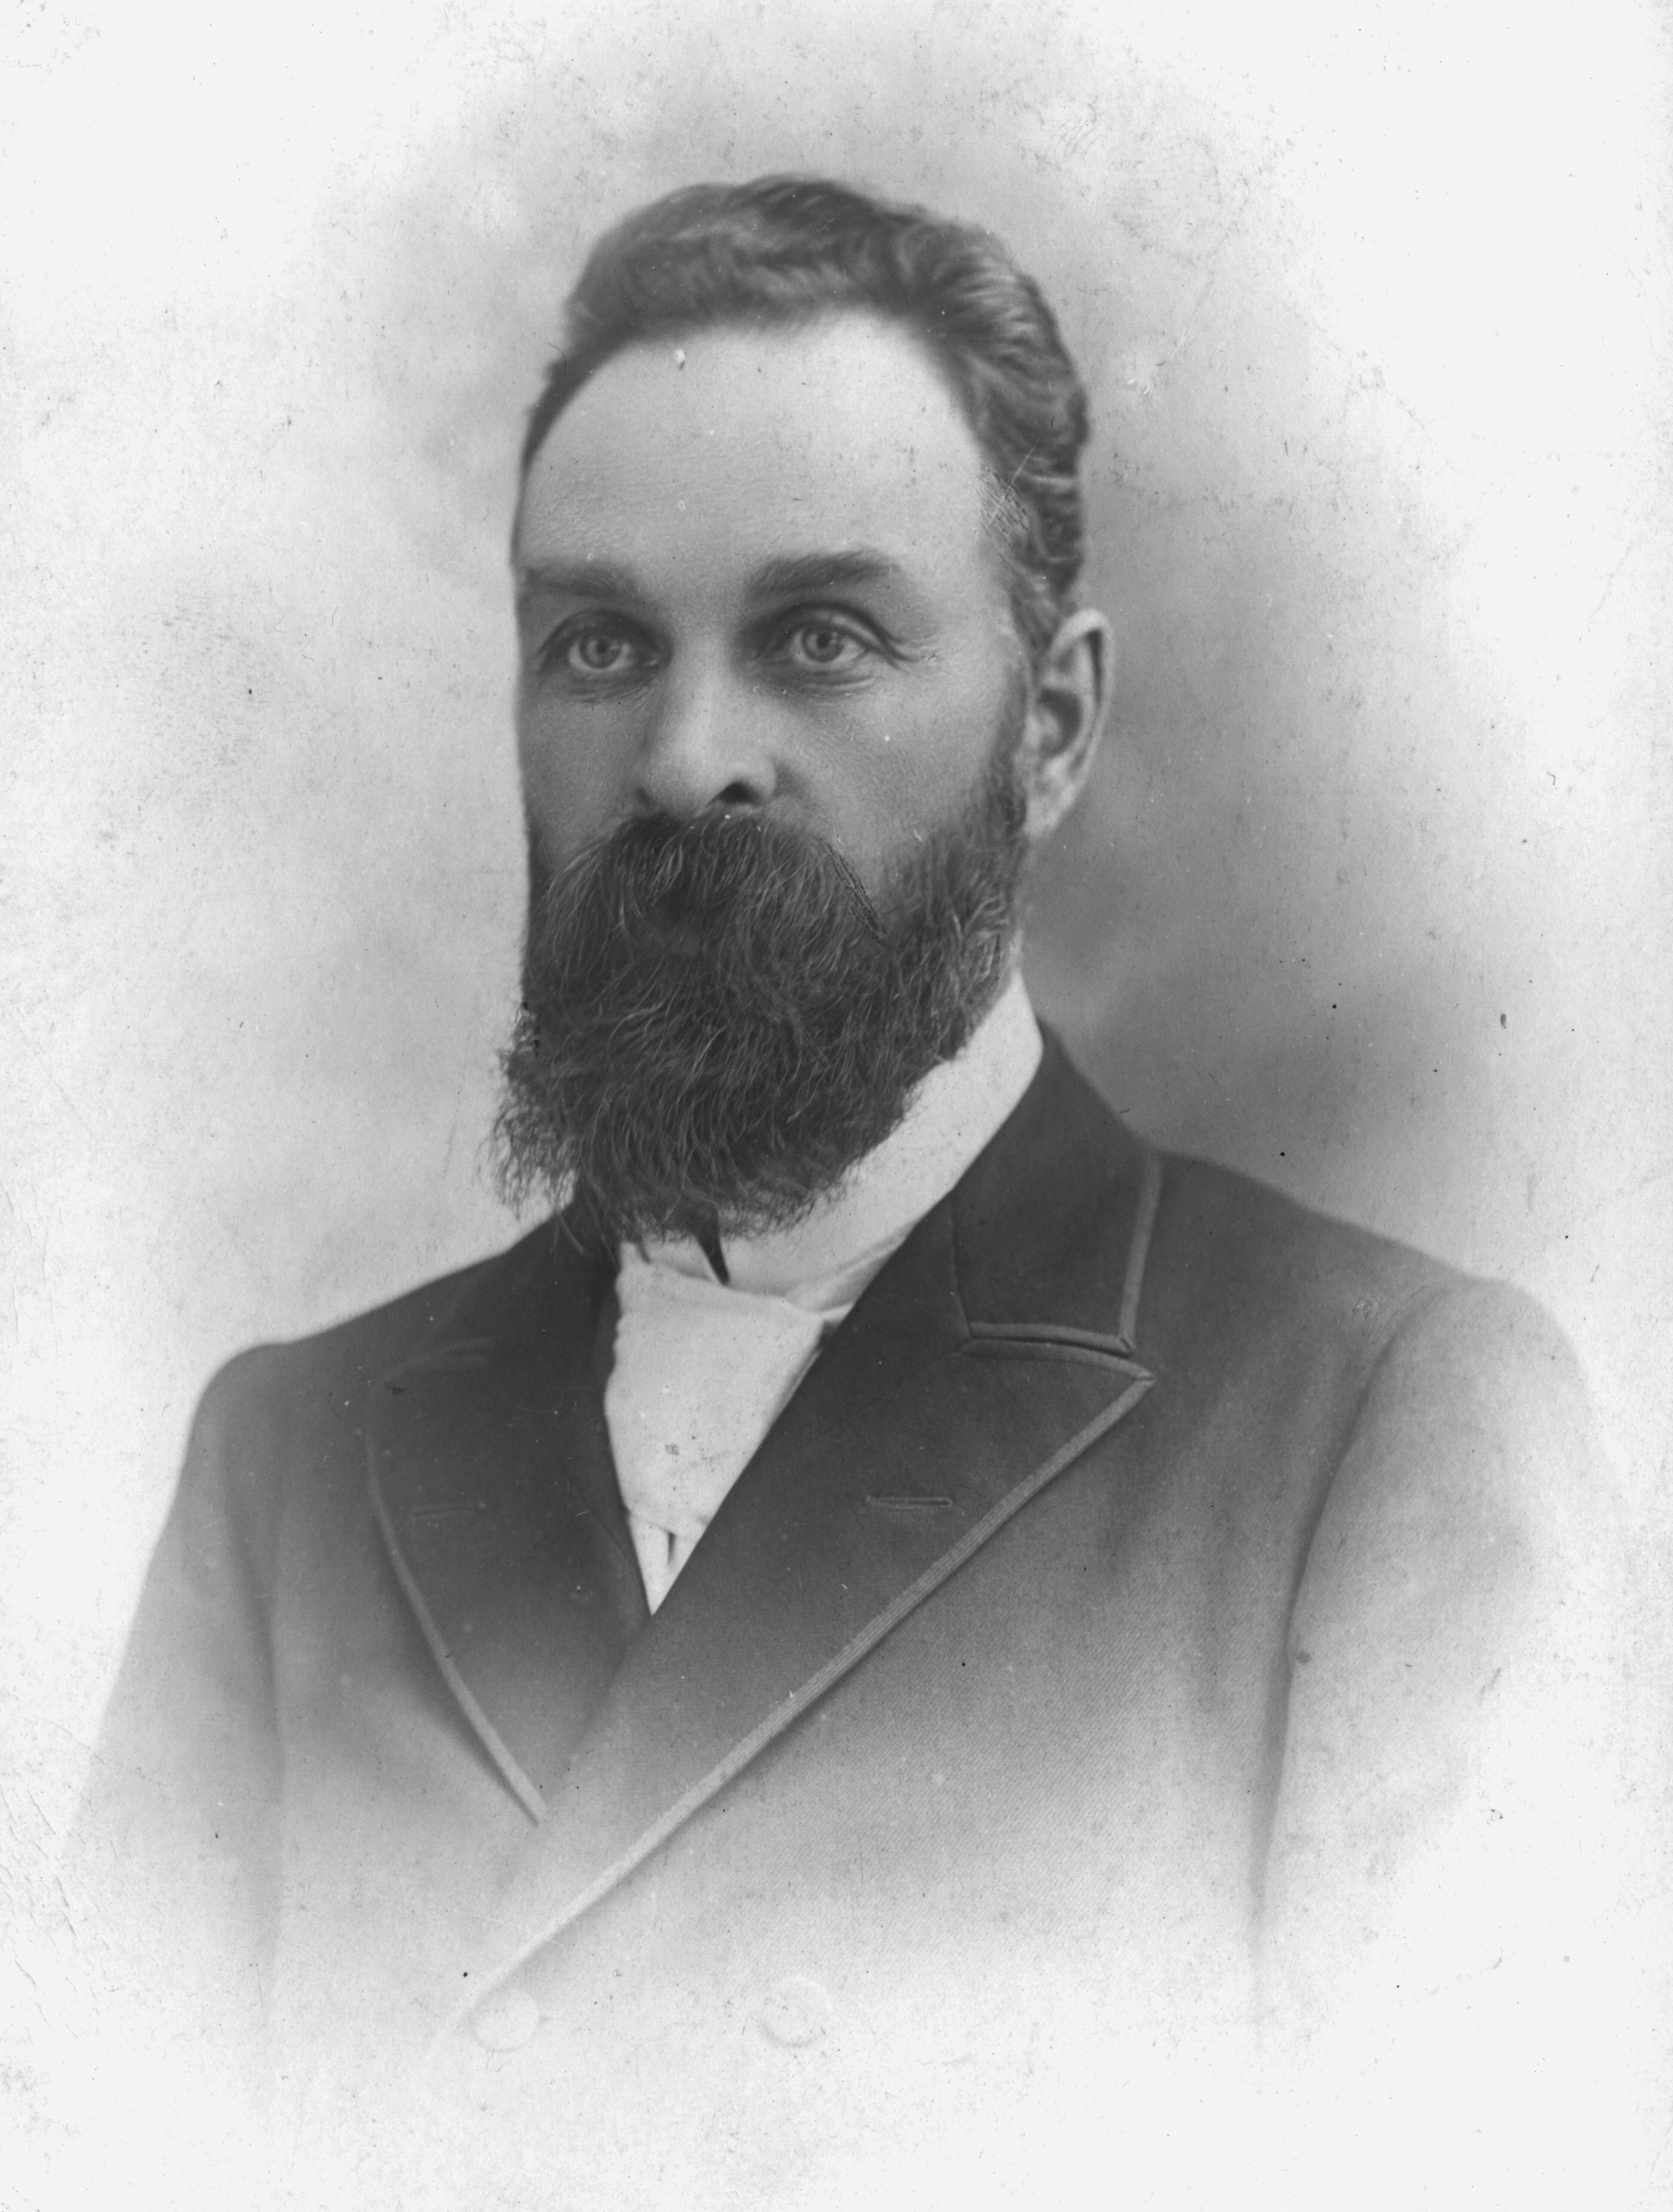
\includegraphics[width=1\linewidth]{images/daniels.jpg}
    \caption*{Arthur Grosvenor Daniells (1858-1935)}
    \label{fig:daniells}
\end{figure}


\othersnogap{\textbf{He then stated that his former views \underline{regarding the trinity} had stood in his way of making a clear and absolutely correct statement; but that within a short time \underline{he had come to believe in the trinity} and could now see pretty clearly where all the difficulty was, and believed that he could clear the matter up satisfactorily.}}


\othersnogap{\textbf{Luego declaró que sus anteriores opiniones \underline{sobre la trinidad} le habían impedido hacer una declaración clara y absolutamente correcta; pero que en poco tiempo \underline{había llegado a creer en la trinidad} y ahora podía ver con bastante claridad dónde estaba toda la dificultad, y creía que podía aclarar el asunto satisfactoriamente.}}


\othersnogap{\textbf{He told me that he now believed in \underline{God the Father, God the Son, and God the Holy Ghost}; and his view was that it was God the Holy Ghost, and not God the Father, that filled all space, and every living thing. He said if he had believed \underline{this} before writing the book, he could have expressed his views without giving the wrong impression the book now gives.}}


\othersnogap{\textbf{Me dijo que ahora creía en \underline{Dios Padre, Dios Hijo y Dios Espíritu Santo}; y que su opinión era que era Dios Espíritu Santo, y no Dios Padre, el que llenaba todo el espacio, y toda cosa viviente. Dijo que si hubiera creído \underline{esto} antes de escribir el libro, podría haber expresado sus puntos de vista sin dar la impresión equivocada que el libro da ahora.}}


\othersnogap{\textbf{I placed before him the objections I found in the teaching, and tried to show him that the teaching was so utterly contrary to the gospel that I did not see how it could be revised by changing a few expressions.}}


\othersnogap{\textbf{Le expuse las objeciones que encontré en la enseñanza, y traté de mostrarle que la enseñanza era tan absolutamente contraria al evangelio que no veía cómo podía ser revisada cambiando unas pocas expresiones.}}


\othersnogap{We argued the matter at some length in a friendly way; but I felt sure that when we parted, the doctor did not understand himself, nor the character of his teaching. And I could not see how it would be possible for him to flop over, \textbf{and in the course of a few days \underline{fix the books up} so that it would be all right}.}[Letter: A. G. Daniells to W. C. White, October 29, 1903. pp. 1, 2][https://forgotten-pillar.s3.us-east-2.amazonaws.com/Letter-A-G-Daniells-to-W-C-White-October-29-1903.pdf]


\othersnogap{Discutimos el asunto largamente de manera amistosa; pero me pareció que cuando nos separamos, el doctor no se entendía a sí mismo, ni el carácter de su enseñanza. Y no pude ver cómo sería posible que él \textbf{se dejara caer, y en el curso de unos pocos días \underline{arreglara los libros} para que todo estuviera bien}.}[Letter: A. G. Daniells to W. C. White, October 29, 1903. pp. 1, 2][https://forgotten-pillar.s3.us-east-2.amazonaws.com/Letter-A-G-Daniells-to-W-C-White-October-29-1903.pdf]


Kellogg did not see the mistake in his sentiments; but rather, in expressing his views. He did not think that his views were false, merely his expression of those views, which led to the book giving a wrong impression. Yet, evidently, this was not true. As Sister White had stated, Kellogg had a problem with the sentiments regarding the \emcap{personality of God} and where His presence is. So, Kellogg suggested that in order to “\textit{fix the books up}” he would include the trinitarian expressions because he now started to believe in \textit{the Trinity} doctrine. At this point in time, the Seventh-day Adventist Church was not trinitarian—the doctrine of Trinity was not part of the \emcap{Fundamental Principles}, as we saw previously. Thus, it is no surprise that Brother Daniels objected and refuted Trinitarian teaching, claiming that it was\others{so utterly contrary to the gospel.} Revising the book, by changing a few expressions, would not change the main problem of the book: the sentiments on the \emcap{personality of God}.


Kellogg no vio el error en sus sentimientos; sino más bien, en la expresión de sus puntos de vista. No creía que sus opiniones fueran falsas, sino que la expresión de las mismas daba lugar a que el libro diera una impresión errónea. Pero, evidentemente, esto no era cierto. Como la hermana White había declarado, Kellogg tenía un problema con los sentimientos relativos a la \emcap{personalidad de Dios} y a dónde está su presencia. Entonces, Kellogg sugirió que para “\textit{arreglar los libros}” incluiría las expresiones trinitarias porque ahora empezaba a creer en la doctrina \textit{trinitaria}. En este momento, la Iglesia Adventista del Séptimo Día no era trinitaria—la doctrina de la Trinidad no era parte de los \emcap{Principios Fundamentales}, como vimos anteriormente. Por lo tanto, no es de extrañar que el hermano Daniels se opusiera y refutara la enseñanza trinitaria, afirmando que era\others{tan absolutamente contraria al evangelio.} Revisar el libro, cambiando algunas expresiones, no cambiaría el problema principal del libro: los sentimientos sobre la \emcap{personalidad de Dios}.


In the described events, and in William White's response to Brother Daniells, we can see why Sister White wrote the Special Testimonies. William White responded to Brother Daniells on Nov. 4, 1903:


En los acontecimientos descritos, y en la respuesta de William White al hermano Daniells, podemos ver por qué la hermana White escribió los Testimonios Especiales. William White respondió al hermano Daniells el 4 de noviembre de 1903:


\others{Dear Brother, --}


\others{Querido hermano, --}


\othersnogap{\textbf{\underline{Mother and I} have just read your letter of \underline{October 29} in which you speak of the \underline{various plans that have been proposed for the revising and reproduction of ‘The Living Temple}.’}}


\othersnogap{\textbf{\underline{Madre y yo} acabamos de leer su carta del \underline{29 de octubre} en la que habla de los \underline{diversos planes que se han propuesto para la revisión y reproducción de ‘El Templo Viviente’}.}}


\othersnogap{We were pleasantly surprised at the announcement that Dr. Kellogg would withdraw this book from the market, \textbf{and we are sorry indeed that his mind is swinging back to the plan of revising it, \underline{Mother expresses herself quite emphatically regarding this matter; she regards it as an unprofitable undertaking}}. I think she will write to you soon expressing her views regarding this.}


\othersnogap{Nos sorprendió gratamente el anuncio de que el Dr. Kellogg iba a retirar este libro del mercado, \textbf{y lamentamos de verdad que su mente esté volviendo al plan de revisarlo, \underline{Madre se expresa con bastante rotundidad respecto a este asunto; lo considera una empresa poco rentable}}. Creo que le escribirá pronto expresando su opinión al respecto.}


\othersnogap{\textbf{… I believe it will be necessary \underline{to issue a special Testimony soon}, and this must contain a very full and clear statement on the positive side of this question, as well as articles pointing out the errors in the teaching of those who have departed from the truth through fascinating and deceptive theories}.}[\href{https://ellenwhite.org/letterbooks/555}{Letter from W.C. White to A.G. Daniells, Nov. 4, 1903,} (p. 458)]


\othersnogap{\textbf{… Creo que será necesario \underline{publicar pronto un Testimonio especial}, y éste debe contener una declaración muy completa y clara sobre el lado positivo de esta cuestión, así como artículos que señalen los errores en la enseñanza de aquellos que se han apartado de la verdad mediante teorías fascinantes y engañosas}.}[\href{https://ellenwhite.org/letterbooks/555}{Carta de W.C. White a A.G. Daniells, 4 de noviembre de 1903,} (p. 458)]


\begin{figure}[h]
    \centering
    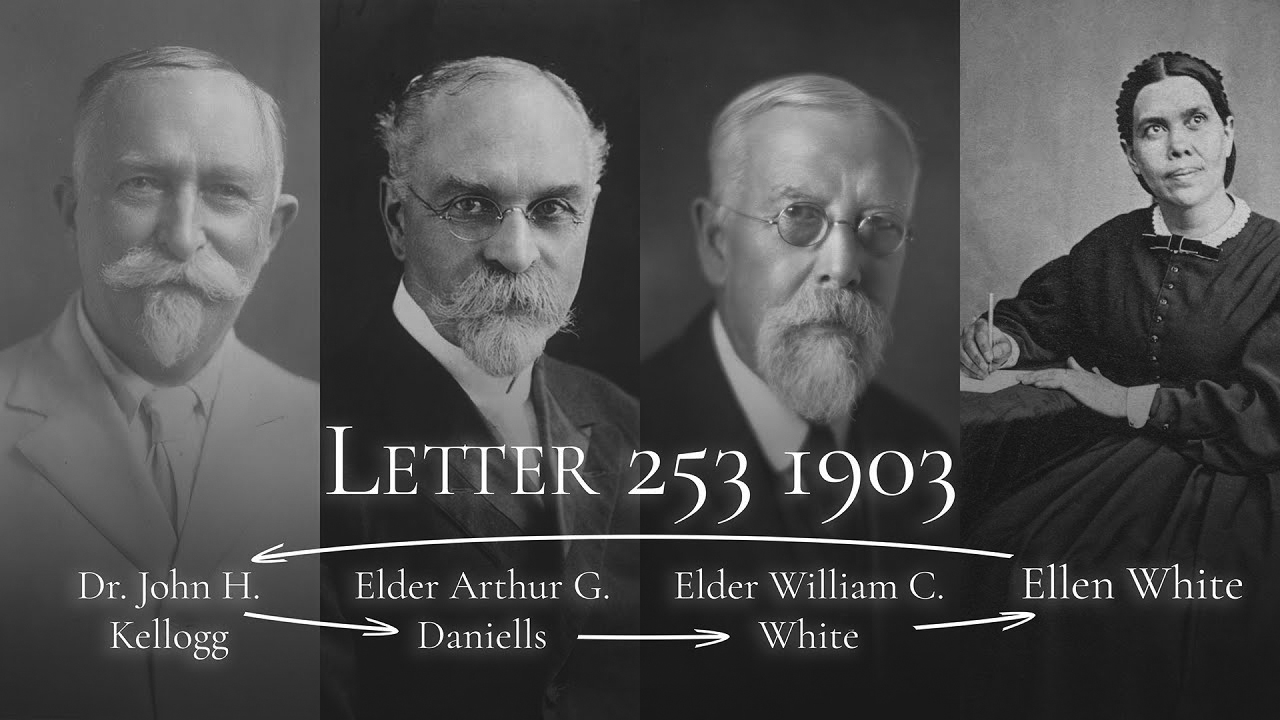
\includegraphics[width=1\linewidth]{images/correspondance.jpg}
    \caption*{Correspondence chain between A. G. Daniells, W. C. White, Ellen White and Dr. John H. Kellogg.}
    \label{fig:corespondance}
\end{figure}


\begin{figure}[h]
    \centering
    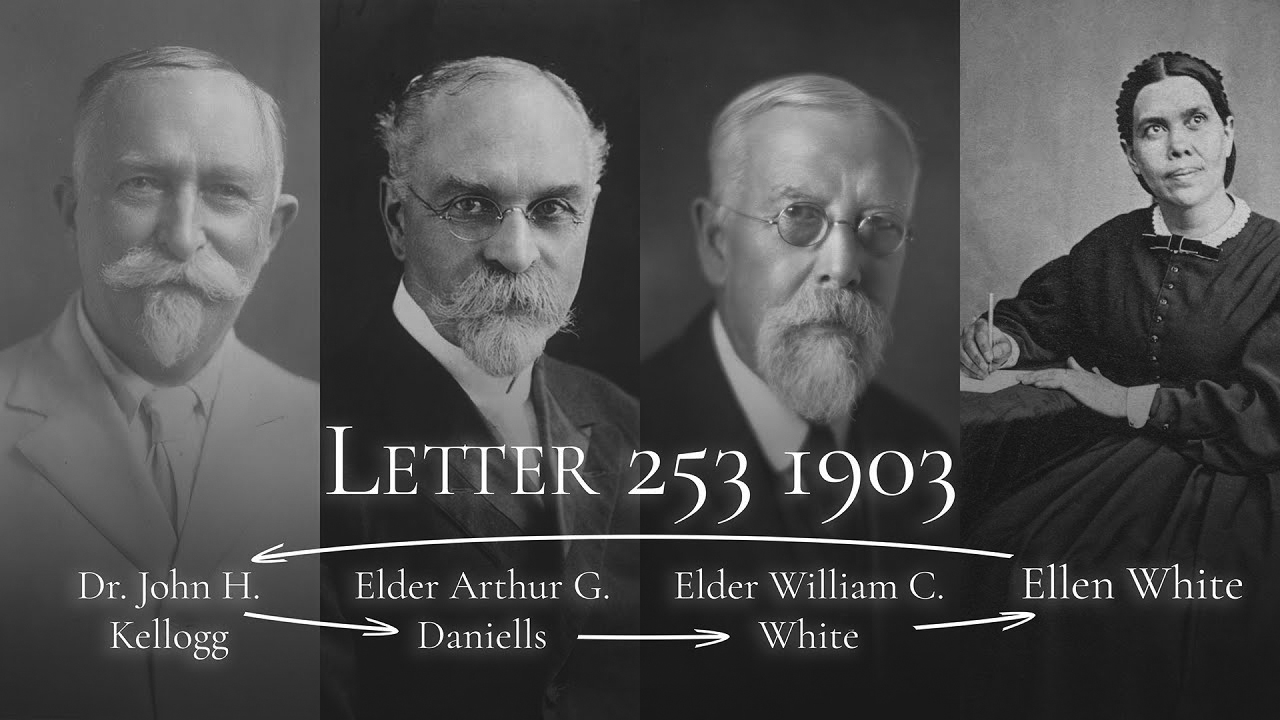
\includegraphics[width=1\linewidth]{images/correspondance.jpg}
    \caption*{Cadena de correspondencia entre A. G. Daniells, W. C. White, Elena G. de White y el Dr. John H. Kellogg.}
    \label{fig:corespondance}
\end{figure}


Here is evidence that Sister White was familiar with Dr. Kellogg's intentions to revise “\textit{Living Temple}” and her familiarity with his belief in the Trinity doctrine. In William's words, she expressed herself quite emphatically regarding this matter. She deemed it an unprofitable undertaking. For this reason, it was necessary to issue a special Testimony soon. And there it was. This is how the \textit{Testimonies for the Church Containing Letters to Physicians and Ministers Instruction to Seventh-Day Adventists} was published in 1904, containing letters to the physicians and ministers connected to Kellogg's crisis.


Aquí hay evidencia de que la hermana White estaba familiarizada con las intenciones del Dr. Kellogg de revisar “\textit{Living Temple}” y su familiaridad con su creencia en la doctrina trinitaria. En palabras de William, ella se expresó con bastante énfasis respecto a este asunto. Lo consideraba una empresa poco rentable. Por esta razón, era necesario emitir pronto un Testimonio especial. Y así fue. Así se publicó en 1904 el \textit{Testimonies for the Church Containing Letters to Physicians and Ministers Instruction to Seventh-Day Adventists}, con cartas a los médicos y ministros relacionados con la crisis de Kellogg.


By saying \others{\textbf{\underline{Mother and I} have just read your letter of \underline{October 29}}}, William testified that Sister White was fully aware of Kellogg's intentions and trinitarian belief. After she read Daniells’ letter, she wrote a direct reply to Dr. Kellogg. This letter is \textit{Lt253-1903}. It is a very prominent and eye opening letter because it clearly exposes how the prophet dealt with the Trinity doctrine. She elevated the doctrine on the \emcap{personality of God} constituted in the \emcap{Fundamental Principles}. There are striking similarities between this letter and the tenth chapter of the Special Testimonies, \textit{The Foundation of our Faith}.


Al decir \others{\textbf{\underline{Madre y yo} acabamos de leer su carta del \underline{29 de octubre}}}, William testificó que la hermana White era plenamente consciente de las intenciones de Kellogg y de su creencia trinitaria. Después de leer la carta de Daniells, escribió una respuesta directa al Dr. Kellogg. Esta carta es \textit{Lt253-1903}. Es una carta muy destacada y reveladora porque expone claramente cómo la profeta trató la doctrina trinitaria. Ella elevó la doctrina sobre la \emcap{personalidad de Dios} constituida en los \emcap{Principios Fundamentales}. Hay sorprendentes similitudes entre esta carta y el décimo capítulo de los Testimonios Especiales, \textit{El Fundamento de Nuestra Fe}.


% Revision of the Living Temple

\begin{titledpoem}
    
    \stanza{
        In Kellogg’s book, a subtle snare \\
        Though well-disguised through crafty care \\
        From Bible truth would lead away \\
        And cause some precious souls to stray.
    }

    \stanza{
        And though much scripture there was used \\
        The early truth became confused \\
        This error served to twist the mind \\
        But in God’s Word the truth we find.
    }

    \stanza{
        God’s personality has form \\
        To Bible truth we must conform \\
        On this the Doctor wasn’t clear \\
        But early Advent truth is dear
    }
    
\end{titledpoem}


% Revision of the Living Temple

\begin{titledpoem}
    
    \stanza{
        In Kellogg’s book, a subtle snare \\
        Though well-disguised through crafty care \\
        From Bible truth would lead away \\
        And cause some precious souls to stray.
    }

    \stanza{
        And though much scripture there was used \\
        The early truth became confused \\
        This error served to twist the mind \\
        But in God’s Word the truth we find.
    }

    \stanza{
        God’s personality has form \\
        To Bible truth we must conform \\
        On this the Doctor wasn’t clear \\
        But early Advent truth is dear
    }
    
\end{titledpoem}
